\documentclass[runningheads]{llncs}

\usepackage[T1]{fontenc}
\usepackage{nicefrac}
\usepackage{amsmath}
\usepackage{amssymb}
\usepackage{booktabs}
\usepackage{multirow}
\usepackage{graphicx}
\usepackage{xcolor}
\usepackage[most]{tcolorbox}
\usepackage{hyperref}
\usepackage[capitalise]{cleveref}
\usepackage{xspace}
\usepackage{enumitem}

\setlength{\emergencystretch}{2em}
\everypar\expandafter{\the\everypar\looseness=-1} % Reduce overfull lines
\linepenalty=1000                                     % Favor fewer line breaks

\newcommand{\ModelName}{\textsc{GNRR}\xspace}

\title{Cross-Document Neural Re-Ranking via Query-Induced Subgraphs}
\author{Anonymous submission}
\institute{}

\begin{document}
\maketitle

% Authors
% ----------------------------------------------------------------------------------
% ==================================================
% Anonymous version for blind peer review
% Keep this active during submission
% ==================================================
\author{Anonymous submission}
\institute{}

% ==================================================
% Authors, uncomment after peer review
% ==================================================
% \author{
% Andrea Giuseppe Di Francesco\inst{1,2}
% \and Christian Giannetti\inst{1}
% \and Nicola Tonellotto\inst{3}
% \and Fabrizio Silvestri\inst{1,3}
% }
%
% \institute{
% Sapienza University of Rome, Rome, Italy
% \email{\{difrancesco,giannetti\}@diag.uniroma1.it}
% \and
% ISTI-CNR, Pisa, Italy
% \and
% University of Pisa, Pisa, Italy
% \email{nicola.tonellotto@unipi.it}
% \email{fsilvestri@diag.uniroma1.it}
% }

% ----------------------------------------------------------------------------------
\begin{abstract}
Neural re-rankers typically score query-document pairs independently, neglecting opportunities to leverage cross-document context within retrieval results.
We propose Graph Neural Re-Ranking (\ModelName), a framework that builds a query-induced subgraph from a pre-computed corpus graph and applies Graph Neural Networks (GNNs) over transformer-based document representations to model inter-document relationships for improved re-ranking.
Unlike self-attention re-rankers that scale quadratically in the number of candidates, \ModelName achieves linear online complexity.
On TREC-DL19, \ModelName achieves a 5.8\% relative improvement in Average Precision over TCT-ColBERT, with consistent gains on DL20 (+3.8\% AP) and DLHard (+5.2\% AP).
GCN-based propagation yields the most robust results across all three benchmarks and all evaluated metrics.
An ablation study confirms that the GNN branch accounts for nDCG@10 improvements of +2.5\% on DL19, +2.2\% on DL20, and
+3.5\% on DLHard, validating that cross-document propagation provides ranking signal beyond what individual query-document
representations capture.
\end{abstract}

\keywords{Neural Re-Ranking, Graph Neural Networks, Corpus Graph}

\section{Introduction}
Modern information retrieval systems typically follow a two-stage pipeline: an initial retrieval step (e.g., BM25 \cite{bm25} or dense retrieval \cite{colbert}) generates a set of candidate documents, which is refined by a neural re-ranking model (e.g., a transformer-based scorer \cite{tctcolbert,vaswani2017attention}) to produce the final ranking.
Despite their effectiveness, most neural re-rankers score each query-document pair independently, discarding relationships among candidates in the retrieved set \cite{monobert,RepBert}.

Capturing cross-document context within the candidate set is desirable but costly. Prior work \cite{pang2020setrank,pobrotyn2020context,pasumarthi2020permutation} has employed self-attention mechanisms over the candidate set, treating documents as a permutation-invariant set \cite{lee2019set,pang2020setrank}. However, self-attention incurs quadratic cost in the number of documents $K$ ($\mathcal{O}(K^2)$), limiting its applicability in latency-constrained settings.

We take a different approach. Rather than attending over all candidate pairs, \ModelName builds a sparse, query-induced subgraph from the retrieved top-$K$ documents using a pre-computed corpus graph \cite{corpusgraph} and applies a lightweight Graph Neural Networks (GNN) to propagate cross-document signals with linear cost $\mathcal{O}(c \cdot K \cdot L)$ where $c$ and $L$ are small constants. Because the corpus graph is pre-computed offline and only a small subgraph is extracted per query, the online computational overhead is substantially reduced compared to dense attention-based approaches.

Our contributions are as follows:
\begin{itemize}
    \item We propose \ModelName, a re-ranking framework that applies GNN-based propagation over query-induced subgraphs to capture cross-document interactions with linear online cost $\mathcal{O}(c \cdot K \cdot L)$ where $c$ and $L$ are small fixed constants. This compares favorably to the $\mathcal{O}(K^2)$ complexity of self-attention-based re-rankers.
    \item We introduce a mechanism to extract query-specific subgraphs from a large pre-computed corpus graph by selecting edges that connect BM25-retrieved candidates, enabling efficient offline-online separation.
    \item We provide a comprehensive empirical analysis of five GNN architectures (GCN, GraphSAGE, GAT, GIN, SignedConv) across three TREC benchmarks with varying difficulty profiles. GCN remains the most stable, achieving up to $\Delta$AP = +5.8\% on DL19, +3.8\% on DL20, and +5.2\% on DLHard. An ablation study confirms that the GNN branch contributes nDCG@10 gains of +2.5\%, +2.2\%, and +3.5\% on the three benchmarks, respectively. 
\end{itemize}

\begin{figure}
    \centering
    
\includegraphics[width=\textwidth]{figures/pipeline_graphical_overview.pdf}
    \caption{Overview of \ModelName ($K=3$). \textit{Offline:} a semantic corpus graph is constructed by computing TCT-ColBERT embeddings over all documents and linking each to its $c$ nearest neighbors. \textit{Online:} given a query, (1) BM25 retrieves top-$K$ candidates; (2) TCT-ColBERT computes embeddings; (3) top-$K$ candidates induce a subgraph from the corpus graph; (4) node features are computed via $f_1(\cdot)$ from query-document embeddings; a GNN propagates cross-document signals to create contextualized representations $f_2(\cdot)$; (5) a learned scorer produces the final ranking. Example: $d_5$ initially ranked 3rd by BM25 but promoted to 1st after GNN re-ranking.}
    \label{fig:overview}
\end{figure}

\section{Related Work}
Transformer-based re-rankers, such as MonoBERT \cite{monobert}, ColBERT \cite{colbert}, and TCT-ColBERT \cite{tctcolbert}. While these models excel at rescoring candidate lists, they either remain too coarse to model inter-document relationships or impose quadratic runtime complexity.

Graph-based representations have long influenced IR research. PageRank \cite{page1999pagerank} exemplifies how linking documents via hyperlinks or citations can improve retrieval quality by propagating importance scores. More recently, MacAvaney et al.\cite{corpusgraph} use a pre-computed corpus graph to expand candidate pools via graph-guided traversal. While prior methods demonstrate the utility of graph structure in early retrieval stages, approaches that leverage trainable graph propagation to directly improve final document ranking remain underexplored.
%In contrast, \ModelName operates within the existing candidate set and applies a trainable GNN to learn which inter-document relationships are discriminative for the re-ranking objective.

GNNs address this gap by jointly learning document representations and propagating relevance signals across the graph, providing a principled mechanism for incorporating corpus-level structure into ranking. GNNs are permutation-invariant \cite{messagepassing,everythingisconnected} and have achieved strong performance across multiple domains \cite{recsystem1,NMT1,VQA}. Early work~\cite{scarselli2005graph} applied GNNs to compute customised PageRanks from labeled examples on web graphs. Subsequent work used GNNs to recover global rankings from pairwise comparisons~\cite{damke2021ranking,he2022gnnrank}, to estimate node importance in complex networks~\cite{liu2022learning,qu2023gnr}, and to rank web resources~\cite{ergashev2023learning}. A separate line of work constructs intra-document word graphs to improve query-document relevance matching~\cite{graphofwords,graphofwords2}. Cross-document structure for re-ranking has been explored only in multi-hop QA~\cite{nie2021answeringanyhopopendomainquestions}; for a broader survey see~\cite{zaoad2025graphbasedrerankingemergingtechniques}. To our knowledge, no prior work applies GNN-based propagation over query-induced subgraphs from a pre-computed corpus graph to improve general-purpose document re-ranking.

\section{Methodology}
\label{sec:methodology}

\ModelName incorporates document-document relationships into neural re-ranking through three stages: (i) offline corpus graph construction, (ii) retrieval and query-induced subgraph extraction, and (iii) GNN-based re-ranking. \cref{fig:overview} illustrates the full pipeline.

\subsubsection*{\textbf{Corpus Graph}}
Given a document corpus $\mathcal{C}$, we construct an offline semantic corpus graph $\mathcal{G} = (\mathcal{C}, \mathcal{E})$ where each document $d \in \mathcal{C}$ is a node and edges $(d_i,d_j) \in \mathcal{E}$ connect semantically similar documents whose cosine similarity in the embedding space exceeds a threshold. Document embeddings $\mathbf{z}_d \in \mathbb{R}^m$ are obtained from TCT-ColBERT \cite{tctcolbert}. Each node's neighborhood is capped at a fixed cardinality $c$ to ensure sparsity and scalability. Although this offline construction is computationally expensive, it is performed only once and the cost is amortised across all queries. To ensure sparsity and scalability, we limit each node's neighborhood to a fixed cardinality $c$.
We follow the construction procedure of \cite{corpusgraph}.

\subsubsection*{\textbf{Retrieval and Subgraph Extraction}}
Given a query $q$, BM25 \cite{bm25} retrieves the top-$K$ documents $\mathcal{C}_q \subseteq \mathcal{C}$. From the corpus graph $\mathcal{G}$, we extract a query-induced subgraph that retains only the retrieved nodes and the edges between them:
\begin{equation} \label{eq:subgraph}
    \mathcal{G}_{q} = (\mathcal{C}_q, \mathcal{E}_q), \quad \mathcal{E}_q = \{(d_i,d_j) \in \mathcal{E} \;|\; d_i,d_j \in \mathcal{C}_q\}.
\end{equation}
Connectivity is bounded by construction: $|\mathcal{E}_q| \leq c \cdot K$. Each node $d_i$ is assigned a feature vector $\mathbf{x}_i = f_1(\mathbf{z}_{q}, \mathbf{z}_{d_i})$, where $\mathbf{z}_{q} \in \mathbb{R}^m$ is the query embedding from TCT-ColBERT. The resulting feature matrix $\mathbf{X}_q \in \mathbb{R}^{|\mathcal{C}_q| \times m}$ encodes query-document relevance independently per node.

\subsubsection*{\textbf{Re-Ranking}}
The GNN operates over the query-induced subgraph $\mathcal{G}_q$ to propagate cross-document signals while preserving each node's individual query-document representation $\mathbf{x}_i$. Each feature vector is augmented with its BM25 score to provide a strong inductive bias and preserve lexical relevance signals. The input to the GNN is thus $\mathbf{X'}_q \in \mathbb{R}^{|\mathcal{C}_q| \times (m+1)}$, which is processed by the GNN to produce contextualized representations:
\begin{equation}
\label{eq:local_interactions}
    \mathbf{H}_{q,\text{GNN}} = \text{GNN}(\mathbf{X'}_q, \mathbf{A}_q),
\end{equation}
where $\mathbf{A}_q$ is the adjacency matrix of $\mathcal{G}_q$ and the hidden dimension is $m'$, yielding $\mathbf{H}_{q,\text{GNN}} \in \mathbb{R}^{|\mathcal{C}_q| \times m'}$.

The contextualized GNN output is merged with the original query-document features through a non-trainable operation $f_2$:
\begin{equation}
    \mathbf{H}_q = f_2\left(\mathbf{H}_{q,\text{GNN}}, \mathbf{X}_q\right).
\end{equation}
A scorer $\phi_{\theta}$ maps $\mathbf{H}_q$ to scalar relevance scores $\mathbf{s}_q \in \mathbb{R}^{|\mathcal{C}_q|}$, producing the final re-ranking:
\begin{equation}
    \pi_q = \text{ARGSORT}(\mathbf{s}_q) = \text{ARGSORT}(\phi_{\theta}(\mathbf{H}_q)).
\end{equation}

\paragraph{Complexity.} Online computation is dominated by the GNN forward pass over $K$ nodes and at most $c \cdot K$ edges, yielding $\mathcal{O}(c \cdot K \cdot L)$ for $L$ GNN layers. Since $c$ and $L$ are fixed constants, online cost scales linearly with $K$. The only computationally intensive step, corpus graph construction, is performed entirely offline.


\section{Experimental Setup}
We address two research questions:
\begin{itemize}[leftmargin=1.1cm]
\item[\textbf{RQ1.}] Does modeling cross-document interactions via GNNs improve re-ranking over a strong transformer baseline?

\item[\textbf{RQ2.}] How much does the GNN branch contribute to the observed gains?
\end{itemize}

\subsection{Datasets}
We use the MS MARCO passage ranking corpus \cite{msmarco}, comprising 8.8 million documents. For training and validation, we sample 1,000 and 200 queries respectively from the MS MARCO training set. While this represents a small fraction of the full training set, these samples are sufficient to learn GNN patterns with LambdaRank\cite{lambdarank}, which is well-calibrated for sparse supervision. Each query has at most one relevant document among the top-1000 retrieved candidates. We evaluate on three standard test sets: TREC-DL19, TREC-DL20 \cite{dl19-20}, and TREC-DLHard \cite{dl-hard}.
\begin{itemize}
    \item \textbf{DL19}: 43 queries, average 215 relevance judgments per query.
    \item \textbf{DL20}: 54 queries, average 211 relevance judgments per query.
    \item \textbf{DLHard}: 50 difficult queries, partially relabeled from DL19 and DL20, targeting topics that challenge neural ranking models.
\end{itemize}

\subsection{Models}
We compare the following pipelines:
\begin{itemize}
    \item \textbf{BM25} \cite{bm25}: lexical retrieval baseline.
    \item \textbf{TCT-ColBERT} \cite{tctcolbert}: transformer-based re-ranker applied on top of BM25, pre-trained on MS MARCO. This serves as the primary baseline for all \ModelName variants.
    \item \textbf{TCT+GCN}: \ModelName with Graph Convolutional Network \cite{GCN}.
    \item \textbf{TCT+GraphSAGE}: \ModelName with GraphSAGE \cite{GraphSAGE}.
    \item \textbf{TCT+GAT}: \ModelName with Graph Attention Network \cite{GAT}.
    \item \textbf{TCT+GIN}: \ModelName with Graph Isomorphism Network \cite{GIN}.
    \item \textbf{TCT+SignedConv}: \ModelName with Signed Graph Convolution \cite{signedconv}.
\end{itemize}
We report four standard IR metrics: Average Precision (AP), Reciprocal Rank (RR), Precision at rank 3 (P@3), and Normalized Discounted Cumulative Gain at rank 10 (nDCG@10). Documents with relevance grade $\\geq 2$ are considered relevant.

\subsection{Training}
All GNN variants are trained with LambdaRank \cite{lambdarank}, a pairwise ranking loss suited to the sparse supervision in MS MARCO, where most queries have a single relevant document. Training runs for up to 100 epochs with early stopping on validation nDCG@10. Only the GNN and scoring modules are updated; the TCT-ColBERT encoders remain frozen. To ensure reproducibility, we commit to releasing complete code, hyperparameter configurations, and preprocessed subgraph data upon acceptance.

\subsection{Hyperparameters}
We set the corpus graph neighborhood size to $c = 8$ and the candidate set size to $K = 1000$, bounding subgraph connectivity at $|\mathcal{E}_q| \leq 8{,}000$ edges. The interaction function is $f_1 = \odot$ (element-wise multiplication) and the merge function is $f_2 = \|$ (concatenation). TCT-ColBERT produces embeddings of dimension $m = 768$. We tune the number of GNN layers $L \in \{1, 2, 3\}$ and hidden dimension $m' \in \{64, 128, 256\}$ via grid search on the MS MARCO validation set, along with architecture-specific hyperparameters (e.g., attention heads for GAT, aggregation function for GraphSAGE, etc.). Optimal configurations vary across datasets, likely due to the different difficulty profiles.

\begin{table}[ht]
    \centering
    \footnotesize
    \caption{Re-ranking performance on TREC-DL19, DL20, and DLHard ($K=1000$). All \ModelName variants (TCT+\{GNN\}) re-rank the same BM25 candidate set using frozen TCT-ColBERT representations. Best score per metric and dataset in \textbf{bold}. Documents with relevance grade $\geq 2$ are considered relevant.}
    \vspace{0.1cm}
    \setlength{\tabcolsep}{3pt}
    \resizebox{\textwidth}{!}{%
    \begin{tabular}{lcccccccccccc}
        \toprule
        \multirow{2}{*}{\textbf{Pipeline}}
            & \multicolumn{4}{c}{\textbf{DL19}}
            & \multicolumn{4}{c}{\textbf{DL20}}
            & \multicolumn{4}{c}{\textbf{DLHard}} \\
        \cmidrule(lr){2-5} \cmidrule(lr){6-9} \cmidrule(lr){10-13}
            & AP & RR & P@3 & nDCG@10
            & AP & RR & P@3 & nDCG@10
            & AP & RR & P@3 & nDCG@10 \\
        \midrule
        BM25
            & 0.286 & 0.642 & 0.473 & 0.480
            & 0.293 & 0.619 & 0.463 & 0.494
            & 0.147 & 0.422 & 0.240 & 0.274 \\
        \addlinespace[2pt]
        +TCT-ColBERT
            & 0.430 & 0.843 & 0.667 & 0.685
            & 0.453 & 0.817 & \textbf{0.691} & 0.680
            & 0.230 & 0.538 & 0.353 & 0.373 \\
        \cmidrule(l){1-13}
        \addlinespace[1pt]
        \quad+GCN
            & \textbf{0.455} & \textbf{0.858} & 0.713 & \textbf{0.702}
            & \textbf{0.470} & \textbf{0.840} & 0.673 & \textbf{0.695}
            & \textbf{0.242} & \textbf{0.559} & \textbf{0.367} & \textbf{0.386} \\
        \quad+GraphSAGE
            & 0.434 & 0.850 & 0.728 & 0.689
            & 0.454 & 0.837 & 0.667 & 0.685
            & 0.223 & 0.531 & 0.366 & 0.379 \\
        \quad+GAT
            & 0.442 & 0.852 & 0.698 & 0.690
            & 0.453 & 0.826 & 0.685 & 0.682
            & 0.219 & 0.542 & 0.364 & 0.376 \\
        \quad+GIN
            & 0.449 & 0.853 & \textbf{0.729} & 0.691
            & 0.455 & 0.793 & 0.642 & 0.675
            & 0.215 & 0.490 & 0.333 & 0.357 \\
        \quad+SignedConv
            & 0.426 & 0.828 & 0.698 & 0.675
            & 0.445 & 0.813 & 0.685 & 0.676
            & 0.218 & 0.509 & 0.353 & 0.366 \\
        \bottomrule
    \end{tabular}%
    }
    \label{tab:benchmarking}
\end{table}

\section{Results}

\subsection*{Contribution of the GNN Branch (RQ2)} 

\cref{fig:ndcg_ablation} isolates the contribution of the GNN branch by comparing each \ModelName variant against the TCT-ColBERT baseline. GCN achieves nDCG@10 improvements of +2.5\% on DL19, +2.2\% on DL20, and +3.5\% on DLHard. This validates the core premise of the framework: learned message passing over query-induced subgraphs provides ranking signal that individual query-document representations do not capture. 

Among the five architectures, GCN consistently outperforms the baseline across all three benchmarks: it achieves the highest AP and nDCG@10 on DL19 (AP $\Delta = +5.8\%$, nDCG@10 $\Delta = +2.5\%$) and DL20 (AP $\Delta = +3.8\%$, nDCG@10 $\Delta = +2.2\%$), and maintains robust performance on the harder DLHard set ($\Delta = +5.2\%$ AP). GraphSAGE and GAT are competitive on DL19 and DL20, but show higher variance on DLHard. GIN and SignedConv suffer larger degradations on DLHard ($-6.5\%$ and $-5.2\%$ relative nDCG@10 respectively), suggesting that simpler, mean-based aggregation (GCN) is more robust when connectivity is sparse and noisy. We attribute GCN's stability to its inductive bias: mean-pooling aggregation acts as a regularizer, preventing the model from overfitting to spurious neighbor relationships in small query-constrained neighborhoods, whereas more expressive operations (attention in GAT, signed edges in SignedConv) struggle to find reliable signal in sparse subgraphs.

These results provide a positive answer to RQ1: modeling cross-document interactions via GNN propagation over query-induced subgraphs yields consistent gains over a strong transformer baseline, with GCN as the most robust variant.

\begin{figure}[t]
  \centering
  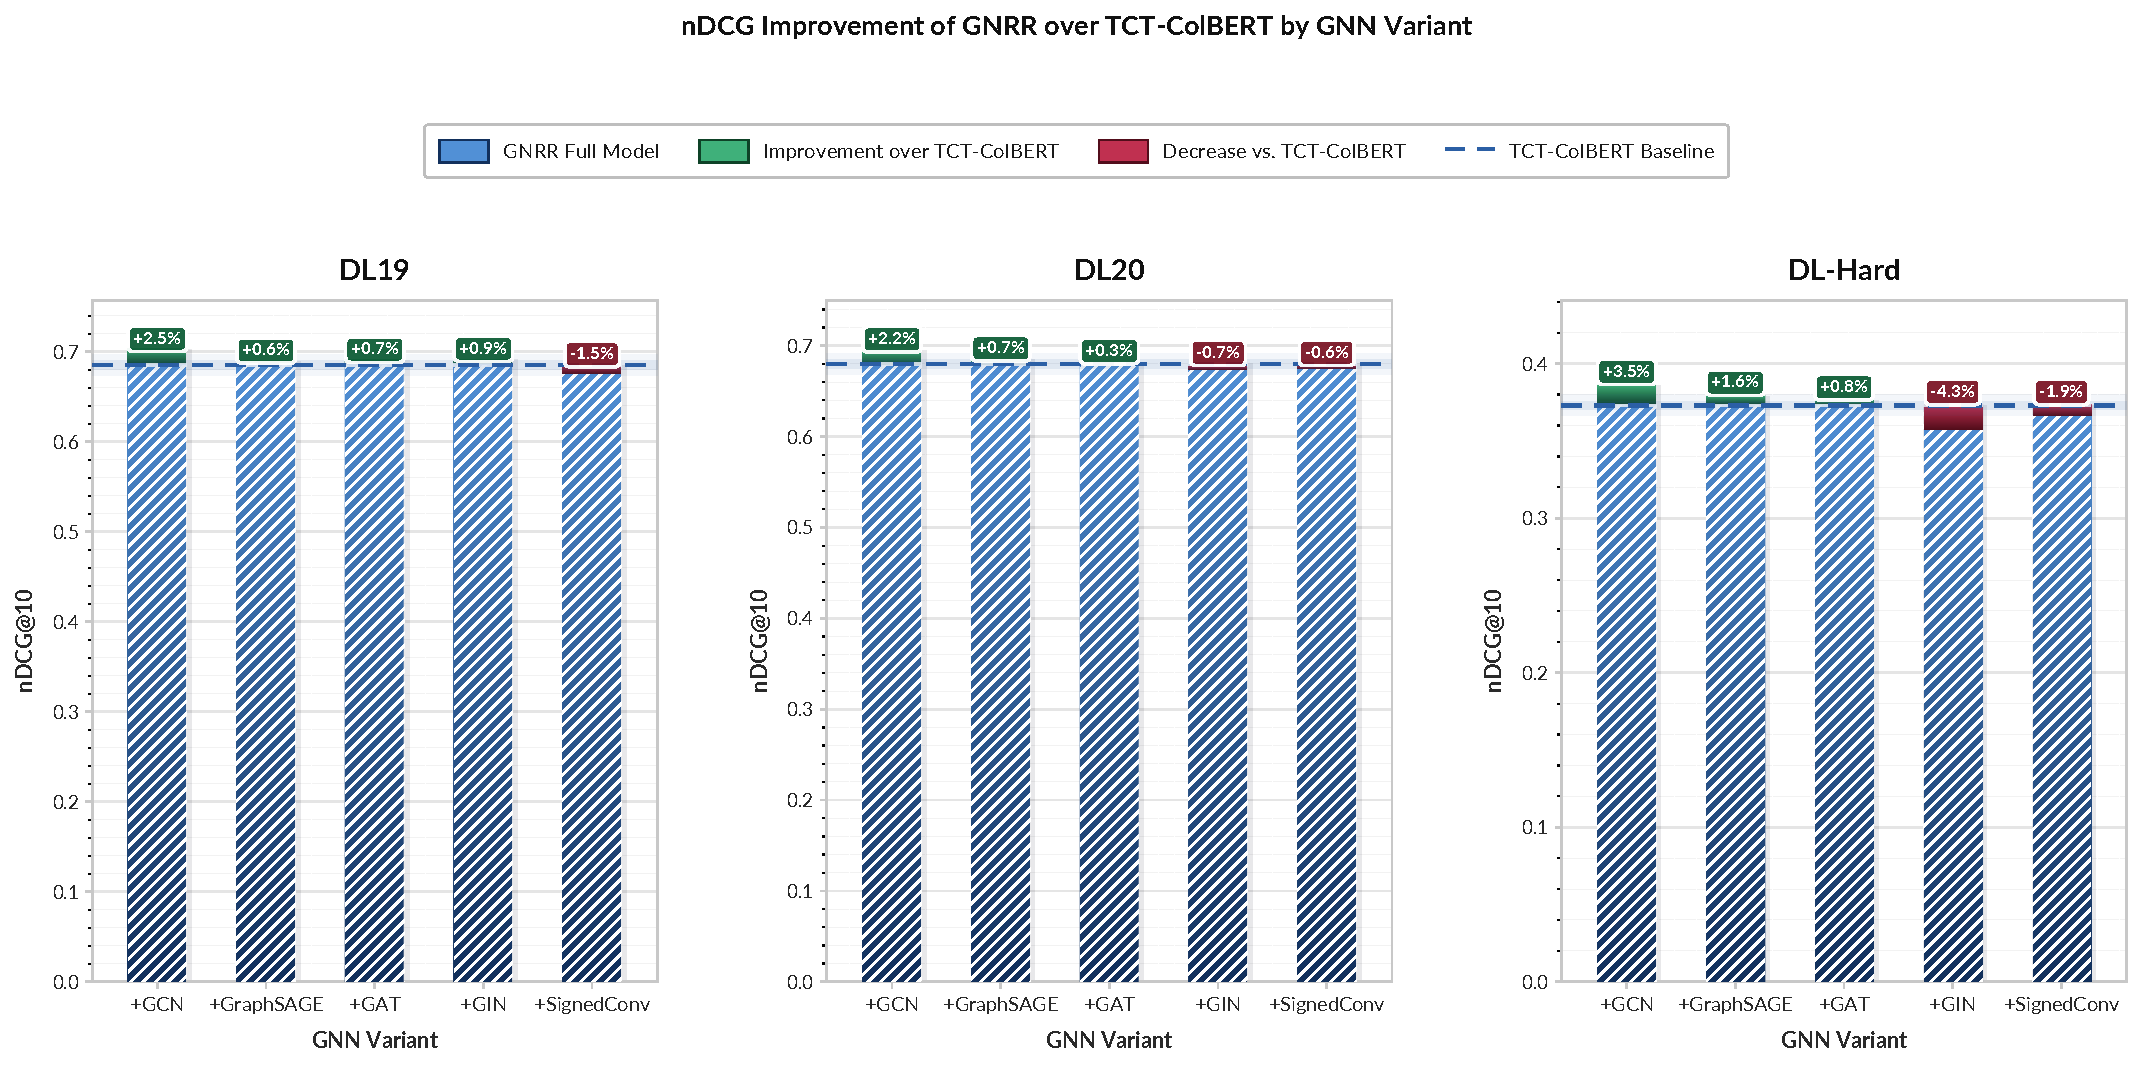
\includegraphics[width=\textwidth]{figures/gnrr_ndcg_updated.pdf}
    \caption{nDCG@10 improvement of each \ModelName variant over the TCT-ColBERT baseline on DL19, DL20, and DLHard. Green caps denote gains; bordeaux caps denote degradation. The dashed line marks the baseline (zero improvement).}
  \label{fig:ndcg_ablation}
\end{figure}

\subsection*{Contribution of the GNN Branch (RQ2)}
\cref{fig:ndcg_ablation} isolates the contribution of the GNN branch by comparing each \ModelName variant against the TCT-ColBERT baseline (i.e., the same pipeline with the GNN branch removed). GCN, the most consistent variant, achieves nDCG@10 gains of +2.5\% on DL19, +2.2\% on DL20, and +3.5\% on DLHard. This validates the core premise of the framework: learned message passing over query-induced subgraphs provides ranking signal that individual query-document representations do not capture.

\section{Conclusions}
This paper introduced \ModelName, a re-ranking framework that captures cross-document interactions by extracting a sparse, query-induced subgraph from a pre-computed corpus graph and applying a GNN on top of transformer-based representations. Unlike self-attention re-rankers with $\mathcal{O}(K^2)$ cost, \ModelName requires only $\mathcal{O}(c \cdot K \cdot L)$ online computation where $c$ and $L$ are small constants. Experiments on TREC-DL19, DL20, and DLHard show that GNN-based propagation yields consistent improvements over a strong TCT-ColBERT baseline. GCN achieves the largest gains across all three evaluation sets, with up to $+5.8$\% relative improvement in Average Precision on DL19 and $+5.2$\% on DLHard. An ablation study confirms that removing the GNN branch degrades nDCG@10 on all three benchmarks, establishing that cross-document propagation provides ranking signal beyond what individual query-document representations capture.

These results establish that sparse inter-document structure via pre-computed corpus graphs is a viable and computationally efficient mechanism for improving neural re-ranking without increasing model complexity at inference time.

\subsection*{Limitations and Future Work}
The current evaluation uses a subset of 1,000 training queries sampled from MS MARCO; scaling to the full training set is a natural next step. The corpus graph is constructed with a fixed neighborhood size ($c=8$) and cosine similarity in TCT-ColBERT embedding space; this design isolates the effect of GNN propagation but leaves open the question of how alternative graph topologies and construction methods influence re-ranking quality.

Future directions include: (1) heterogeneous graph structures encoding queries, entities, and diverse relation types (e.g., clicks, citations, co-citations); (2) alternative dense retrieval encoders (e.g., ColBERTv2, ANCE) to study how encoder capacity interacts with graph-based propagation; (3) adaptive, query-specific graph construction in place of fixed topology; and (4) evaluating whether cross-document propagation is complementary to other re-ranking strategies.
\begin{credits}
\subsubsection{Generative AI Usage Disclosure}
Generative AI tools were used for debugging assistance and language editing only. Conceptualization, methodology, experimental design, analysis, and manuscript writing were conducted entirely by the authors.

\subsubsection{\discintname}
The authors have no competing interests to declare that are relevant to the content of this article.
\end{credits}

%
% ---- Bibliography ----
%
% BibTeX users should specify bibliography style 'splncs04'.
% References will then be sorted and formatted in the correct style.

\bibliographystyle{splncs04}
\bibliography{main}

\end{document}
